\documentclass[hidelinks,12pt,a5paper,openright,twoside]{book}
\usepackage[italian]{babel}
\usepackage[utf8]{inputenc}
\usepackage{fourier}

% To avoid GitHub Action error
\usepackage{hyperref}

%To loop a command
\usepackage{forloop}

% Stop hyphenation
\usepackage[none]{hyphenat}

% Adjust paragraph.
\usepackage{changepage}
\usepackage{geometry}

% Background page image.
\usepackage{eso-pic}

% Images
\usepackage{graphicx}
\usepackage{caption}
\usepackage{subcaption}
\usepackage{float}
\graphicspath{ {../Notebook_cover} }

\usepackage{xcolor}

% License
\usepackage[
type={CC},
modifier={by-nc-sa},
version={4.0},
]{doclicense}

\newcounter{lines}
\newcommand{\insertLines}[1]{ % Generate multiple lines from a number
														% Argument -> number of lines
	\forLoop{1}{#1}{lines}{
		 \line(1,0){\linewidth}
	}
}


\newcommand{\normalPage}{% Page composed of only lines
	\begin{adjustwidth}{-10mm}{0mm}
		\centering
		\par \line(1,0){\linewidth}
		\insertLines{34}
		\newpage
	\end{adjustwidth}
}

\newcommand{\topNotationPage}[1]{% Page where curiosity are on the top
	\begin{adjustwidth}{0mm}{-10mm}
		\centering
		\fboxrule=2pt
		\fbox{
			\par
			\begin{minipage} [l] [\dimexpr .250\textwidth \relax] [t] {\dimexpr 0.9\textwidth \relax}
				\textbf{\large Lo sapevi?}\\
				#1
			\end{minipage}
		}
		\bigskip
		\par \line(1,0){\linewidth}
		\insertLines{28}
	
		\newpage
	\end{adjustwidth}
}

\newcommand{\bottomNotationPage}[1]{% Page where curiosity are on the bottom
	\begin{adjustwidth}{-10mm}{0mm}
		\centering
		\par \line(1,0){\linewidth}
		\insertLines{26}
		\\
		\bigskip
		\fboxrule=2pt
		\fbox{
			\begin{minipage} [l] [\dimexpr .250\textwidth \relax] [t] {\dimexpr 0.9\textwidth \relax}
				\textbf{\large Lo sapevi?}\\
				#1
			\end{minipage}
		}
		
		\newpage
	\end{adjustwidth}
}

\pagestyle{empty}

\begin{document}
	\newgeometry{top=15mm, bottom=15mm}
	
		%Notebook cover
		\begin{adjustwidth}{0mm}{-8.8mm}
			\begin{center}
			\vspace*{15mm}
			\textcolor{lightgray}{\fboxrule=4pt{
				\fbox{ %                                                          height                                width
					\begin{minipage}[l] [\dimexpr 0.150\textwidth \relax] [t] {\dimexpr .600\textwidth \relax}
						\vspace{2mm}
						\centering{\large \textbf{Notebook con curiosità sulle opere dei Musei\\}}
						\vspace{10mm}
						Francesco Rombaldoni
					\end{minipage}
				}
			}}
		\end{center}
	\end{adjustwidth}
	
		% Background image
		\AddToShipoutPictureBG*{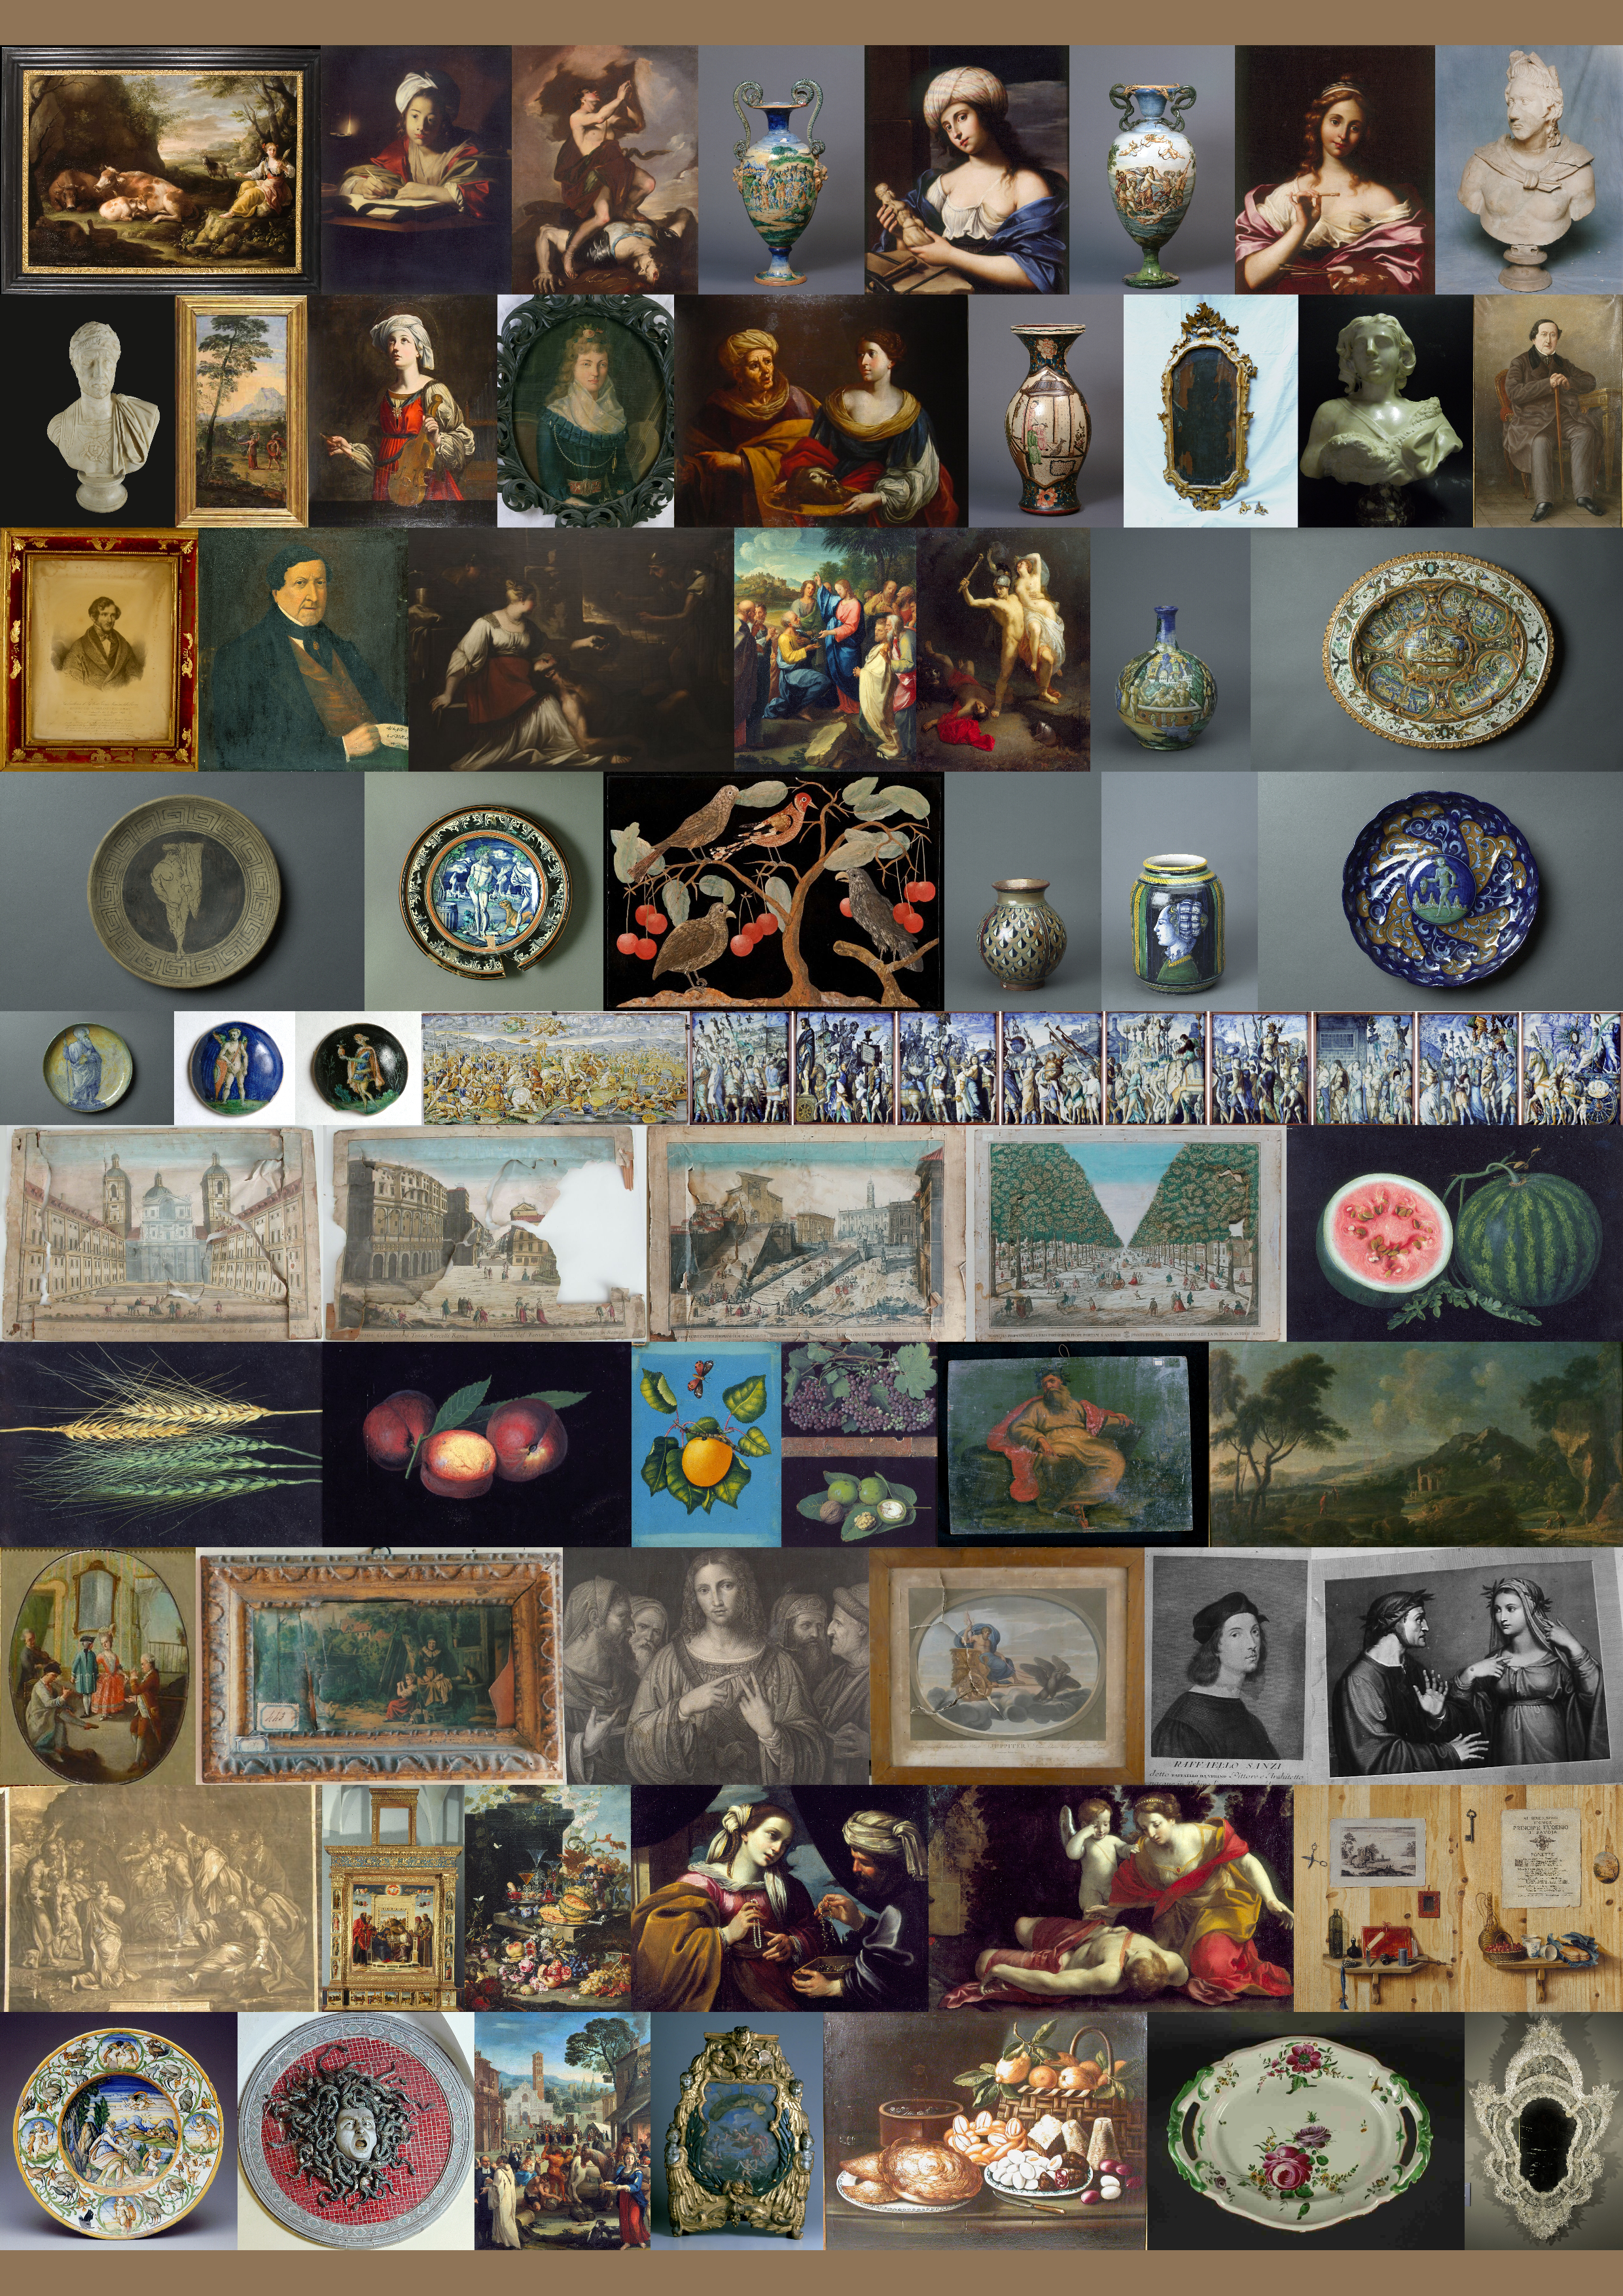
\includegraphics[ width=\paperwidth,height=\paperheight]{Cover.png}}
		\newpage
	
		\normalPage
		
		\topNotationPage{\footnotesize Si dice che la Medusa in ceramica di Mengaroni porti sfortuna. Mentre l'artista la creava guardandosi allo specchio, questo si ruppe: un presagio della sua futura morte, avvenuta proprio cercando di salvare l'opera che stava scivolando.}
		
		\normalPage
		
		\bottomNotationPage{La Pala di Giovanni Bellini non è un semplice quadro. È dipinta come un'opera nell'opera: la cornice dipinta e quella reale si fondono, e la scena può essere letta sia in orizzontale che in verticale.}
		
		\normalPage
		
		\topNotationPage{La parte superiore (Cimasa) della Pala del Bellini fu rubata da Napoleone. Fu recuperata solo grazie all'intervento di Antonio Canova e oggi si trova ai Musei Vaticani, non a Pesaro!}
		
		\normalPage
		
		\bottomNotationPage{Nei quadri antichi, come quelli della collezione Ercolani-Rossini, il rosso brillante dei panneggi veniva estratto da insetti essiccati (i "vermi", da cui vermiglio). Un colore decisamente "naturale"!}
		
		\normalPage
		
		\topNotationPage{La Marchesa Mosca soffriva d'insonnia. Il suo "Orologio Notturno" proiettava l'ora sul muro grazie a una candela interna, permettendole di sapere che ore fossero senza alzarsi dal letto.}
		
		\normalPage
		
		\bottomNotationPage{Le ceramiche "Belle Donne" erano i "social media" del Rinascimento. I nobili regalavano piatti con il ritratto dell'amata e la scritta "Bella" per corteggiarle o celebrare le nozze.}
		
		\normalPage
		
		\topNotationPage{La Beata Michelina, protettrice di Pesaro, disse: "La mia città tremerà ma non cadrà". Una frase che i pesaresi ricordano ogni volta che la terra trema.}
		
		\normalPage
		
		\bottomNotationPage{San Terenzio, patrono di Pesaro, nella Pala del Bellini è vestito da soldato romano. È raro: solitamente viene rappresentato come un vescovo anziano o un giovane con la palma del martirio.}
		
		\normalPage
		
		\topNotationPage{Alcune ceramiche dei Musei Civici brillano come oro o rubino. È grazie alla tecnica del "lustro", una terza cottura segreta con fumi di ginestra e rosmarino, tipica di Deruta e Gubbio.}
		
		\normalPage
		
		\bottomNotationPage{Ferruccio Mengaroni era così bravo a imitare la maiolica rinascimentale che spesso i critici scambiavano le sue opere moderne per pezzi autentici del Cinquecento!}
		
		\normalPage
		
		\topNotationPage{Un bassorilievo ai Musei Civici mostra i profili di Battista Sforza e Federico da Montefeltro. Nonostante fossero parenti acquisiti (lei nuora della matrigna di lui), il loro fu un matrimonio felice e colto.}
		
		\normalPage
		
		\bottomNotationPage{Il quadro di Guido Reni mostra i giganti cacciati dall'Olimpo. È un'opera così dinamica che sembra quasi si possa sentire il frastuono della caduta guardando i corpi intrecciati.}
		
		\normalPage
		
		\topNotationPage{La Marchesa Vittoria Toschi Mosca non collezionava solo arte, ma viveva letteralmente dentro il museo. Lasciò tutto alla città affinché i giovani artigiani potessero ispirarsi al bello.}
		
		\normalPage
		
		\bottomNotationPage{Il quadro "Morte di Adone" è stato a lungo un mistero. Attribuito a Sementi, poi a Guido Reni, poi declassato ad anonimo nel 1993. Un vero cold case della storia dell'arte!}
		
		\normalPage
		
		\topNotationPage{Nelle maioliche istoriate, spesso i paesaggi di sfondo non sono reali, ma scenari fantastici con rovine romane aggiunte per dare un tono solenne ed epico alla scena.}
		
		\normalPage
		
		\bottomNotationPage{Il Museo Oliveriano custodisce una mappa del 1508 circa che è tra le prime al mondo a riportare la scritta "Mundus Novus" (Nuovo Mondo) sulle coste del Sud America. Una "breaking news" del XVI secolo!}
		
		\normalPage
		
		\topNotationPage{La famosa Stele di Novilara mostra una battaglia navale o un atto di pirateria. È la prova che i Piceni non erano solo agricoltori, ma temibili marinai dell'Adriatico.}
		
		\normalPage
		
		\bottomNotationPage{Una delle stele di Novilara contiene un'iscrizione in "Nord Piceno" che nessuno è ancora riuscito a decifrare completamente. È il codice segreto dell'archeologia locale!}
		
		\normalPage
		
		\topNotationPage{\footnotesize L'Anemoscopio di Boscovich è un disco di marmo romano unico nel suo genere. Serviva a orientarsi con i venti e forse a fare calcoli astronomici. Olivieri lo amava così tanto da volerlo all'ingresso per testamento.}
		
		\normalPage
		
		\bottomNotationPage{Nel bosco sacro (Lucus Pisaurensis) sono stati trovati ex-voto in terracotta a forma di piedi, mani e occhi. Erano le richieste di guarigione degli antichi romani alle divinità.}
		
		\normalPage
		
		\topNotationPage{Tra i reperti c'è un askos (vaso) a forma di scarpa. Curioso oggetto di design dell'antichità, probabilmente usato per versare oli o profumi durante i rituali.}
		
		\normalPage
		
		\bottomNotationPage{I mosaici delle domus romane di Pesaro raffigurano spesso delfini e mostri marini. Pesaro (Pisaurum) è sempre stata una città legata indissolubilmente al mare.}
		
		\normalPage
		
		\topNotationPage{La fibula di Verucchio con inserti in ambra testimonia che già nell'antichità esistevano "autostrade" commerciali che collegavano il Baltico all'Adriatico.}
		
		\normalPage
		
		\bottomNotationPage{La Tabula Fabrorum è una lastra di bronzo che dimostra come i fabbri romani di Pesaro avessero una loro corporazione (sindacato) molto potente, devota alla dea Minerva.}
		
		\normalPage
		
		\topNotationPage{Molti sarcofagi romani del museo sono sopravvissuti perché nel Medioevo venivano usati come abbeveratoi per animali o vasche per fontane. Il riciclo creativo li ha salvati!}
		
		\normalPage
		
		\bottomNotationPage{La Biblioteca Oliveriana contiene oltre 400.000 volumi. Se li mettessimo in fila, coprirebbero chilometri di cultura, partendo dagli incunaboli del 1400.}
		
		\normalPage
		
		\topNotationPage{Sotto le navi della Stele di Novilara ci sono delle spirali. Gli archeologi pensano rappresentino le onde del mare agitate durante la battaglia.}
		
		\normalPage
		
		\bottomNotationPage{Nelle tombe femminili di Novilara sono state trovate vesti con centinaia di pendagli in bronzo e pasta vitrea. Camminando, queste donne dovevano "suonare" a ogni passo!}
		
		\normalPage
		
		\topNotationPage{Annibale degli Abati Olivieri, che donò la collezione, era un nobile illuminato. Scoprì il Lucus Pisaurensis quasi per caso, seguendo la sua passione per l'antiquariato.}
		
		\normalPage
		
		\bottomNotationPage{Sulla Tabula Fabrorum c'è Minerva. Non solo dea della guerra, ma protettrice dell'intelligenza e delle arti manuali, perfetta patrona per i fabbri.}
		
		\normalPage
		
		\topNotationPage{Gioachino Rossini, nato a Pesaro, era famoso tanto per le sue opere quanto per il suo appetito. I "Maccheroni alla Rossini" e il "Tournedos Rossini" sono invenzioni nate dalla sua passione culinaria.}
		
		\normalPage
		
		\bottomNotationPage{Pesaro è la città della bicicletta. La sua metropolitana di superficie non ha treni, ma piste ciclabili colorate che collegano tutta la città (linea blu per il mare, verde per il parco...).}
		
		\normalPage
		
		\topNotationPage{Pesaro è stata Capitale Italiana della Cultura 2024, un riconoscimento che ha celebrato la sua unione unica tra natura (il parco San Bartolo) e tecnologia (la Sonosfera).}
		
		\normalPage
		
		\bottomNotationPage{È un anfiteatro tecnologico unico al mondo per l'ascolto profondo. Lì dentro puoi sentire il suono delle foreste equatoriali come se fossi in Amazzonia.}
		
		\normalPage
		
		\topNotationPage{Sul colle San Bartolo c'è Villa Imperiale, capolavoro del Rinascimento. Fu costruita in due fasi: una per la difesa (Sforza) e una per il piacere (Della Rovere), incastrate tra loro.}
		
		\normalPage
		
		\bottomNotationPage{Pesaro è Città Creativa UNESCO per la Musica, non solo per Rossini, ma per la presenza di uno dei conservatori più antichi e prestigiosi d'Italia.}
		
		\normalPage
		
		\topNotationPage{Prima dei Romani, a Verucchio e dintorni c'erano i Villanoviani (antenati degli Etruschi). I reperti oliveriani mostrano quanto fossero avanzati nella lavorazione dei metalli.}
		
		\normalPage
		
		\bottomNotationPage{Il vero nome è "Sfera Grande". È diventata il punto di ritrovo per eccellenza dei pesaresi: "Ci vediamo alla Palla". È una copia dell'originale che si trova alla Farnesina a Roma.}
		
		\normalPage
		
		\topNotationPage{Molte ceramiche del museo vengono da "Casteldurante". Oggi questa città si chiama Urbania, ma ha mantenuto la tradizione della maiolica di altissimo livello.}
		
		\normalPage
		
		\bottomNotationPage{Il nome romano della città deriva probabilmente dal fiume Foglia, anticamente chiamato Pisaurus. I Romani fondarono la colonia nel 184 a.C.}
		
		\normalPage
		
		\topNotationPage{Uno stile di ceramica si chiama "Raffaellesco" perché ispirato alle decorazioni (grottesche) scoperte nella Domus Aurea e rese famose da Raffaello Sanzio.}
		
		\normalPage
		
		\bottomNotationPage{Insieme alla Beata Michelina, fondò la confraternita per assistere gli infermi. Pesaro nel '300 era un centro molto attivo di carità francescana.}
		
		\normalPage
		
		\topNotationPage{Pesaro passò sotto lo Stato Pontificio nel 1631. I pesaresi ricordano ancora i moti e le proteste storiche legate alle tasse sul sale imposte dai papi.}
		
		\normalPage
		
		\bottomNotationPage{Su una coppa ai Civici è dipinta la caccia al Cinghiale Calidonio. Un mito greco cruento trasformato in un elegante oggetto da tavola per le corti rinascimentali.}
		
		\normalPage
		
		\topNotationPage{Francesco Xanto Avelli, ceramista famoso, era anche un poeta e un uomo colto che firmava le sue opere. Una vera "archistar" della maiolica del Cinquecento.}
		
		\normalPage
		
		\bottomNotationPage{Nella predella della Pala Bellini, San Girolamo legge nel deserto. Ma se guardate bene, il "deserto" assomiglia molto alle colline marchigiane!}
		
		\normalPage
		
		\topNotationPage{Il Teatro Rossini di Pesaro è rinomato per la sua acustica. Fu inaugurato nel 1818 con "La Gazza Ladra" diretta dallo stesso Rossini.}
		
		\normalPage
		
		\bottomNotationPage{Oltre alla Biblioteca Oliveriana, Pesaro vanta un patrimonio musicale immenso conservato presso la Fondazione Rossini, meta di studiosi da tutto il mondo.}
		
		\normalPage
		
		\topNotationPage{Camminando per il centro, spesso si calpestano mosaici romani che si trovano pochi metri sotto il livello stradale attuale. Gli scavi continuano a rivelare sorprese!}
		
		\normalPage
		
		\bottomNotationPage{\footnotesize La testa della Medusa all'ingresso dei Musei Civici non è una donna, ma un autoritratto! L'artista Ferruccio Mengaroni si scolpì guardandosi allo specchio mentre urlava, per catturare la perfetta espressione di terrore.}
	
		\newpage
		\vspace*{\fill}
		% Print license shield
		\textcolor{white}{\textbf{\doclicenseThis}}
		% Background image
		\AddToShipoutPictureBG*{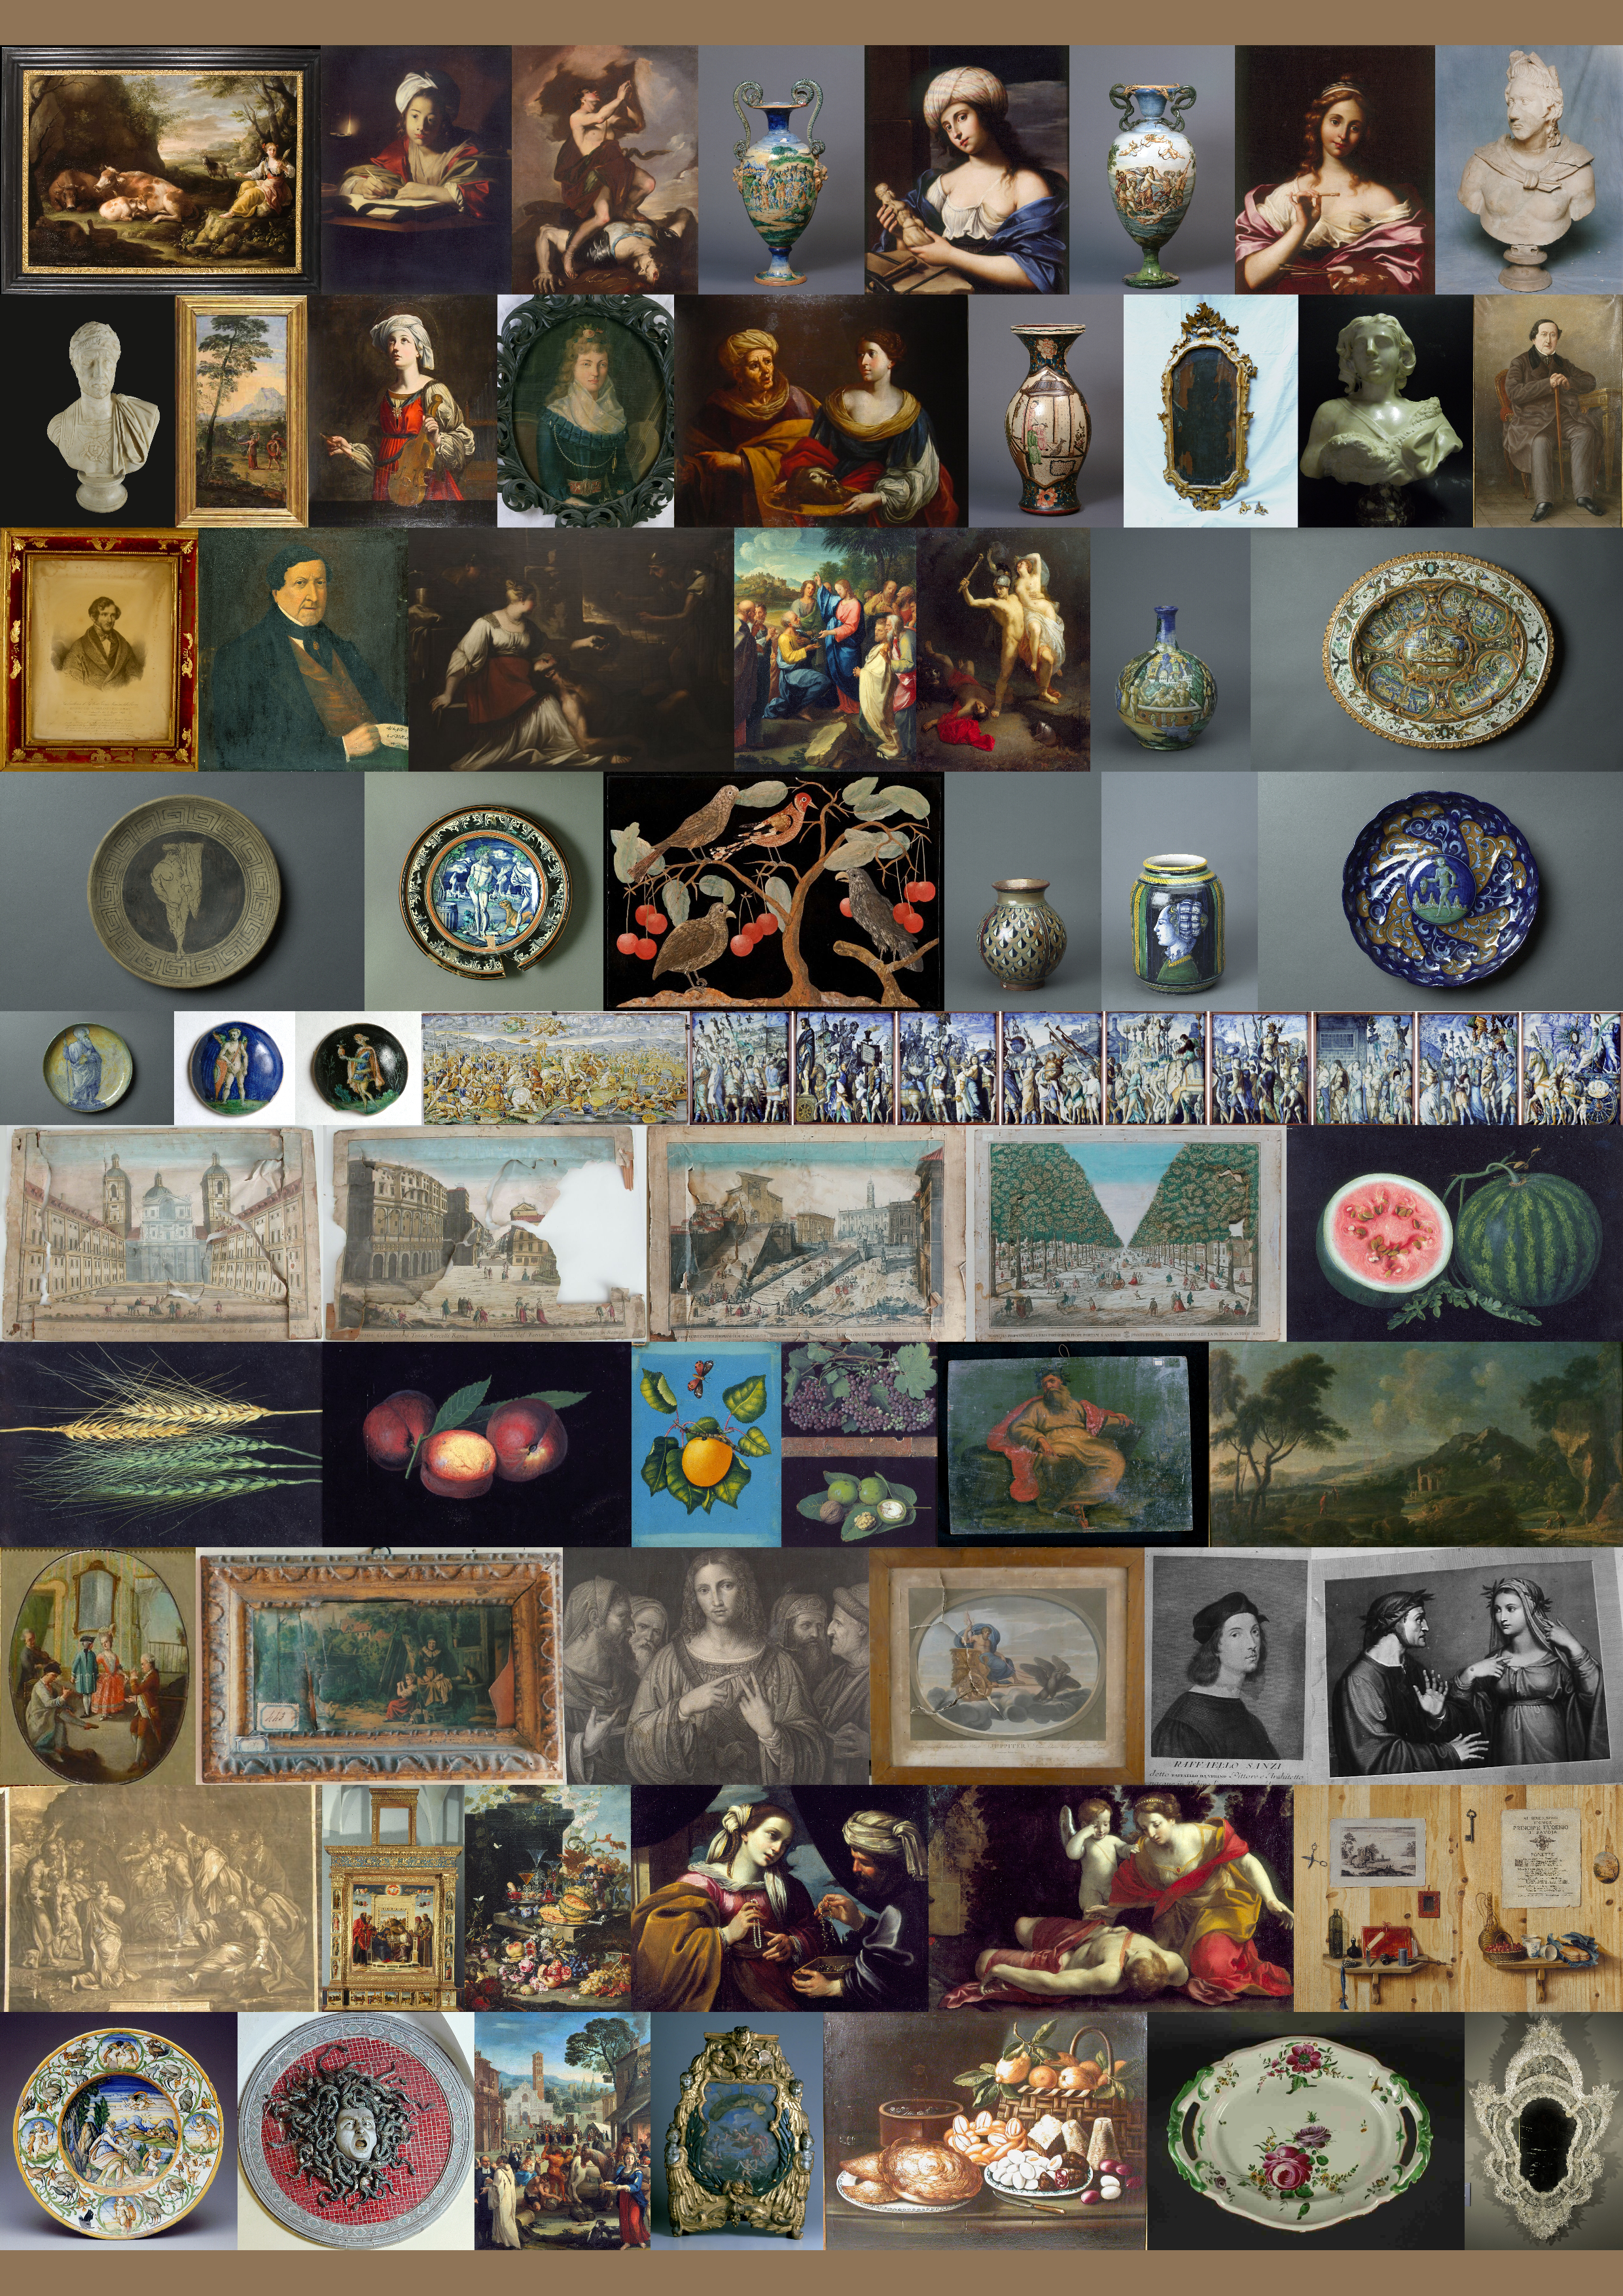
\includegraphics[ width=\paperwidth,height=\paperheight]{Cover.png}}
\end{document}
